\chapter{Experimental work and result in mode I}
\label{Chapter3}

\section{Introduction}

In this chapter, the opening mode failure behaviour is investigated using the DIC method. We present and analyse the force vs the crack opening curve obtained with the DIC method and python code.  Then the evolution of the crack length curves along the x-axis is obtained as a function of displacement. Finally, the energy restitution rates for the MMCG specimens are calculated and analysed with some other articles.

\section{Experimental set-up}

\subsection{Camera and MatchiD setup}
An x-camera coupled with a 60mm Nikkor lens was used for image acquisition. The camera has a resolution of x (H) × x (V) and a sensor size of x. The front of the lens was positioned at a working distance of 285 mm with an aperture of f/11 and an exposure time of 60 milliseconds. The displacement of the machine was 0.02mm/s and the camera had a frequency of 1 Hz, i.e. 1 frame per second.

add speckle pattern DIC+ histogram

The kinematic fields acquired by image correlation (e.g., subset size, subset step, ldots) and numerical differentiation (e.g., strain windows size) algorithms can be significantly impacted by the DIC configuration settings. Since they will determine the spatial resolution and accuracy linked to the DIC measurements, both in displacement and strain fields, these settings constitute fundamental parameters.  In order to balance resolution and spatial resolution, a parametric research was done to support the DIC setting for the current application. The MatchID 2D Parametric Module was used to conduct this investigation.

\begin{table}[]
	\centering
	\begin{tabular}{c c}
		\hline
		Correlation   Coefficient: & ZNSSD \\ 
		Interpolation order: & Bicubic Splines \\ 
		Transformation order: & Quadratic \\
		Subset size: & 31 \\
		Step size: & 10 \\
		Strainwindow size: & 5 \\ 
		Strain interpolation: & Q4 \\ 
		Strain Convention: & Green-Lagrange \\ \hline
	\end{tabular}
	\caption{MatchID parameters used}
	\label{tab:MatchID_param}
\end{table}

The range of values defined in this performance study, including the subset size ($f_s$), subset step, affine and quadratic displacement shape functions, the size of the strain windows, and the order of the polynomial fitting function, is defined by the table \ref{tab:MatchID_param}. It is believed that the pre-selected range of values is reflective of the permissible DIC setup parameter range.

\subsection{Hydraulic press and arcan system setup}

The Landmark Servohydraulic compression tensile machine, with a capacity of 100 kN, can be seen in Figure \ref{fig:Setup0°}. The camera and Arcan device are also clearly visible. The part of the specimen with the speckle pattern was illuminated so that the black dots could be correctly distinguished for image correlation. The camera was mounted on a tripod in order to capture stable images during the tests. The movable jaw of the test machine is controlled in fixtures and is equipped with a load sensor.
The hydraulic press was set up by Mr Martins. The first step was to adjust the distance between the two parts of the press in order to be able to place our specimen with the arcan system. The bolts figure \ref{fig:fig25}  were then placed on the press. Between each test, the arcan system with the specimen was attached to the bolts. Washers were placed between the specimen and the Arcan system to reinforce the hole attachments. To change specimen between two tests, manual controls were used to raise the moving part of the press and avoid residual tension between the bolt hole and the arcan system. An arbitrary preload was also applied to the specimen before the start of the test, to prevent any specimen movement. The position and load are given each time by the MTS software controller. In addition, a plot is created in real time. It was important to stop the press if too many tests were carried out, to avoid overheating the oil/water supplying the hydraulic press. Overheating can cause problems such as the moving part of the press rising or falling rapidly, destroying a specimen without capturing any images. This is what happened to one of the specimens.

\begin{figure}[htp]
	\centering
	\includegraphics[width=12cm]{Setup0°}
	\caption{Experimental set-up}
	\label{fig:Setup0°}
\end{figure}

\subsection{MMCG specimen last preparation}

All the specimens have been painted to obtain a pattern that allows image processing as explained above. MatchID requires spots to be made up of a given number of pixels. A first layer of white paint was added and a cloud of black dots formed a second layer of paint. All the paints used are matt paints, not gloss paints. The dimensions of the painted areas are not precisely defined. It is not necessary to paint the heels, as they have not been studied. The pattern is also different for each specimen, but a black dot is about 10 pixels long. A scale has been added to specimen e0e6, for example, in order to convert the pixels into mm and then measure the crack length. 

\begin{figure}[htp]
	\centering
	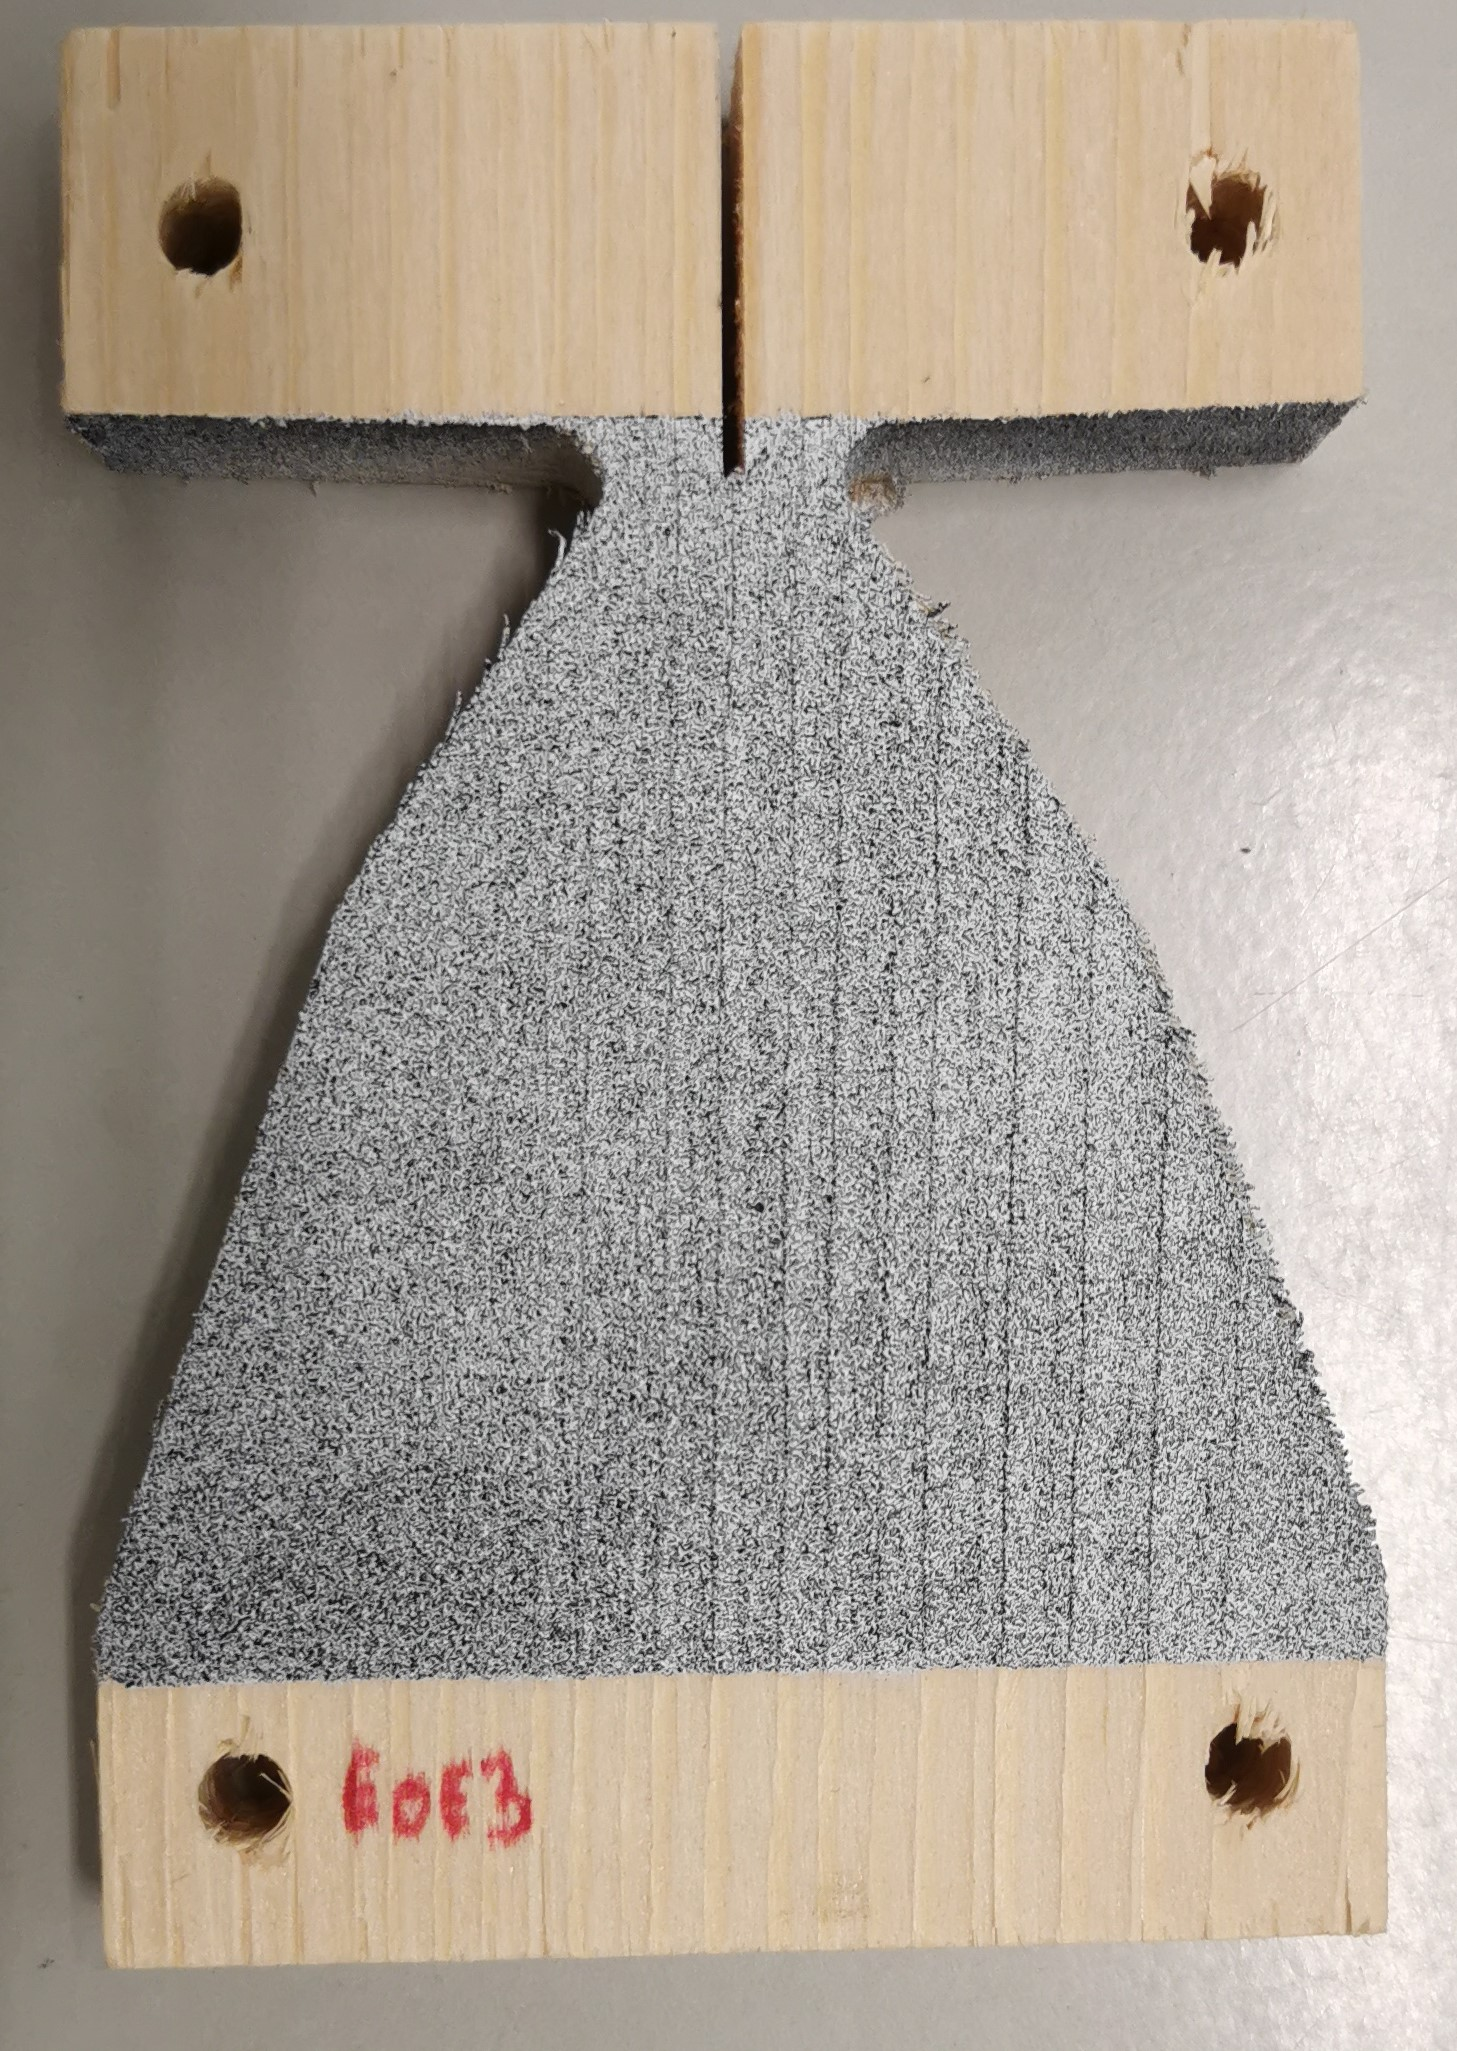
\includegraphics[width=4cm, angle=90]{Speckle_pattern}
	\caption{Speckle pattern obtained for each sample}
	\label{fig:Speckle_pattern}
\end{figure}

\section{Force-displacement curve}

Normally four distinct parts are observed on a force-displacement curve:

\begin{itemize}
	\item A small area visible at the beginning of the curve which corresponds to the setting up of the loaded specimen. 
	\item A practically linear zone, terminated by the critical force FC , due to the elastic part of the loading with a static crack front.
	\item A third part characterised by the observation of a set of critical force peaks FC responsible for a fairly clear initiation of the crack. The increasing peaks validate the zone of stability of the crack.
	\item Finally, a last part where the rupture of the material occurs following the application of a breaking force translating the final instability of the crack.
\end{itemize}

 In the figure \ref{fig:e0e1_Pdelta}, we don't see the setting up of the loaded specimen because a slight preload has been applied to the specimen so that it does not move during the beginning of the test. In addition, it is also quite difficult to see the critical FC force peaks because of the noise caused by the load sensor.

\begin{figure}[htp]
	\centering
	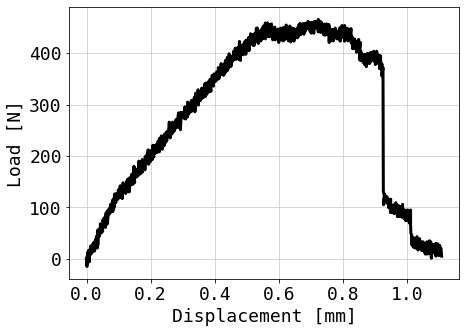
\includegraphics[width=9cm]{e0e1_Pdelta}
	\caption{Characteristic P-Delta curve}
	\label{fig:e0e1_Pdelta}
\end{figure}


\section{Deformation maps}

Typical deformation map ($\epsilon$yy) obtained with the DIC method is shown in Figure \ref{fig:Strain_def}.
During the tests we noticed that the cracks tend to propagate according to the orientation and inclination of the fibres.
In figure \ref{fig:Strain_def} for specimen e0e1, we assume a small fibre inclination which could explain the crack orientation that we see.

\begin{figure}[htp]
	\centering
	\begin{tabular}{c}
		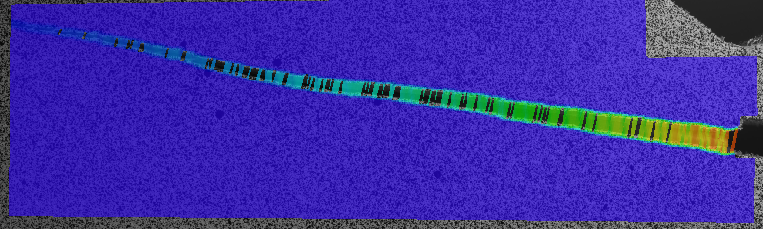
\includegraphics[width=8cm]{e0e1} \\
		e0e1 deformation map \\
		\\
		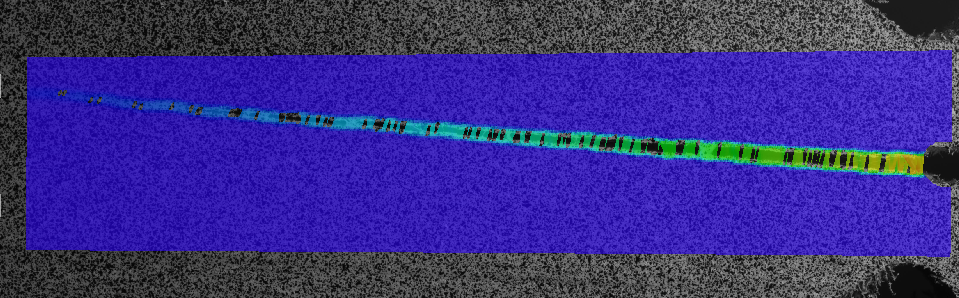
\includegraphics[width=8cm]{e0e2} \\
		e0e2 deformation map \\
		\\
		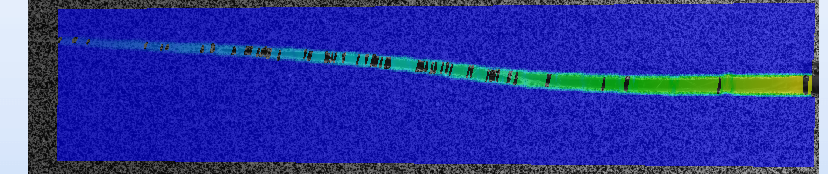
\includegraphics[width=9cm]{e0e3} \\
		e0e3 deformation map \\
	\end{tabular}
	\caption{Typical deformation map ($\epsilon$yy) obtained with DIC}
	\label{fig:Strain_def}
\end{figure}

Strain maps are used to best locate the position of the crack tip by graphic reading.
Thus, thanks to the deformation maps we are able to obtain the crack length on different stages. It is then possible to check whether method 1 and method 2 are working correctly.
The blue points figure \ref{fig:fig39} and \ref{fig:fig40} for tests e0e1 and e0e2 are the points read graphically with the deformation maps. We can see that the blue points follow the curves of method 1 and method 2 correctly, so we can consider that both methods are working correctly. However, it seems that method 1 is slightly more accurate.

\begin{figure}[htp]
	\begin{minipage}[c]{.46\linewidth}
		\centering
		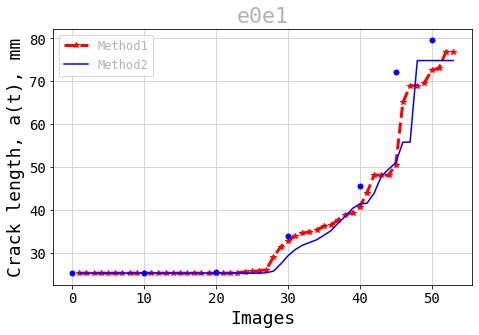
\includegraphics[width=7cm]{e0e1_graphicread}
		\caption{Crack tip by graphic reading e0e1}
		\label{fig:fig39}
	\end{minipage}
	\hfill%
	\begin{minipage}[c]{.46\linewidth}
		\centering
		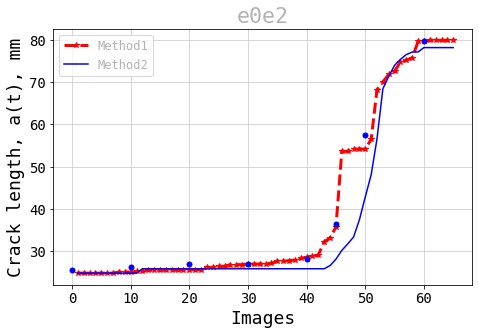
\includegraphics[width=7cm]{e0e2_graphicread}
		\caption{Crack tip by graphic reading e0e2 }
		\label{fig:fig40}
	\end{minipage}
\end{figure}


\section{Force - Crack tip opening curve}

The user must select the "CODpair". In order to provide accurate displacement, the chosen pair of subsets must be as close as possible to the crack tip while yet being sufficiently removed to prevent information loss (if they are positioned inside the crack). Databases are updated using the selected CODpair following this study. Due to the selected COD pair being in blue, a plot was produced that displays the wI shapes that were used, as seen on figure \ref{fig:CTOD_example}. In order to demonstrate for each specimen that the COD pair picked could not have been more exact, the plot also compared this curve to the one created using the lower and upper COD pairs.

\begin{figure}[htp]
	\centering
	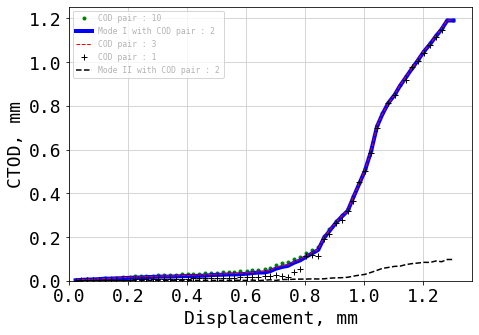
\includegraphics[width=9cm]{CTOD_example}
	\caption{Crack Tip Opening Displacement}
	\label{fig:CTOD_example}
\end{figure}

All the crack opening curves in mode I (displacement of the two lips of the crack) are shown in figure \ref{fig:COD_modeI}. 
We can see two distinct phases in these curves. A first phase in which the force increases with a slight increase of the CTOD and a second phase in which the load decreases with a sharp increase of CTOD. In the first phase, the MMCG specimen resists the force applied by the tensile machine, whereas in the second phase, the crack is already well initiated. There is therefore little resistance for the wood sample, which explains why the force decreases and the COD increases.

\begin{figure}[htp]
	\centering
	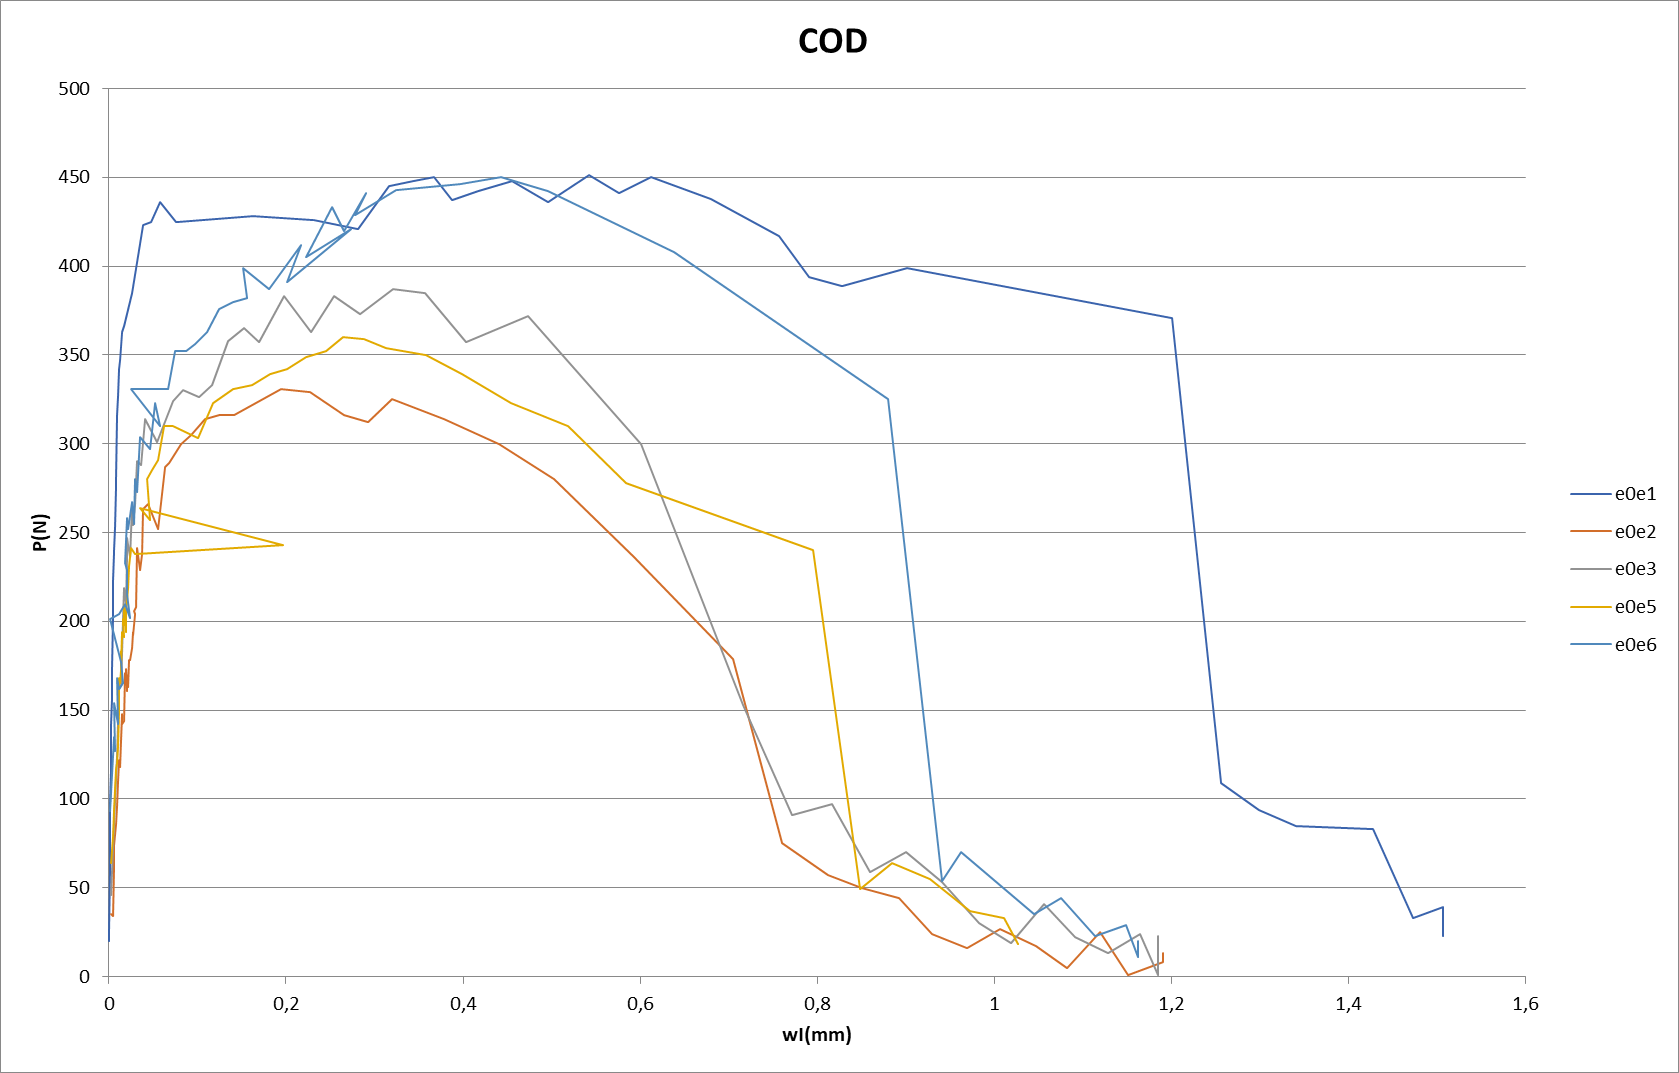
\includegraphics[width=16cm]{COD_modeI}
	\caption{Crack Opening Displacement}
	\label{fig:COD_modeI}
\end{figure}

\section{Crack length-Displacement curve}

For method 1 by compiling the evolution of a(t) as a function of the images recorded for several alpha values (\ref{fig:CTOD_example}), it is possible to get an idea of the alpha value required to obtain the best a(t). Indeed, the alpha parameter must be as small as possible for the evolution of the crack length to be complete. So, for each crack length in the sample, it is possible to eliminate several candidates. In this example \ref{fig:CTOD_example}, it is possible to eliminate the use of curves with a(t)<70mm. These alpha values do not allow the entire crack length to be studied. To distinguish between the black and turquoise curves, you can use the displacement map by placing the position of the crack tip with a red dot on a figure. For different stages, we can then see which curve corresponds best to the position of the crack tip. Here, the black curve was chosen.

To obtain a(t) using method 2, we need to read $a_1$ and $a_f$ graphically and choose a pair of COD lines that are not damaged by nans values.

\begin{figure}[htp]
	\centering
	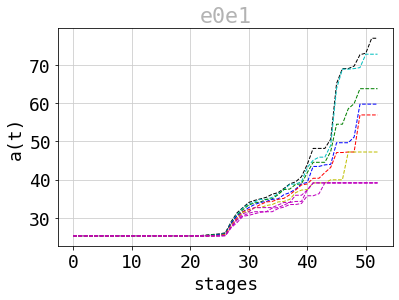
\includegraphics[width=9cm]{Cracklength_modeI_example}
	\caption{Crack length evolution depending on alpha}
	\label{fig:Cracklength_modeI_example}
\end{figure}

All the crack length curve in function of displacement in mode I are shown in figure \ref{fig:crack_method1} and \ref{fig:crack_method2}. 
With method 1, there are, as expected, different plateaus for the crack length.The crack length increases gradually and continuously before rupture. It is the design of the MMCG specimen that allows the stable propagation of the crack. Indeed, with this specimen, cracks progress slowly until failure occurs at maximum load. In some images, bridges prevent the fracture from propagating linearly. When these bridges break, the crack propagates, involving a new stage. It is interesting to examine all the crack length propagation plots.  The curves are all more or less the same shape, and the crack ends at roughly the same length. What differs is the stage at which the crack begins to propagate. For example, we can see that e0e1 begins its crack propagation at stage 23, whereas e0e2 begins at stage 9.
As for method 2, it gives broadly the same curves as the method 1 but the curve is smoother, which is not necessarily a good thing since crack propagation in wood normally works more step by step.

\begin{figure}[htp]
	\centering
	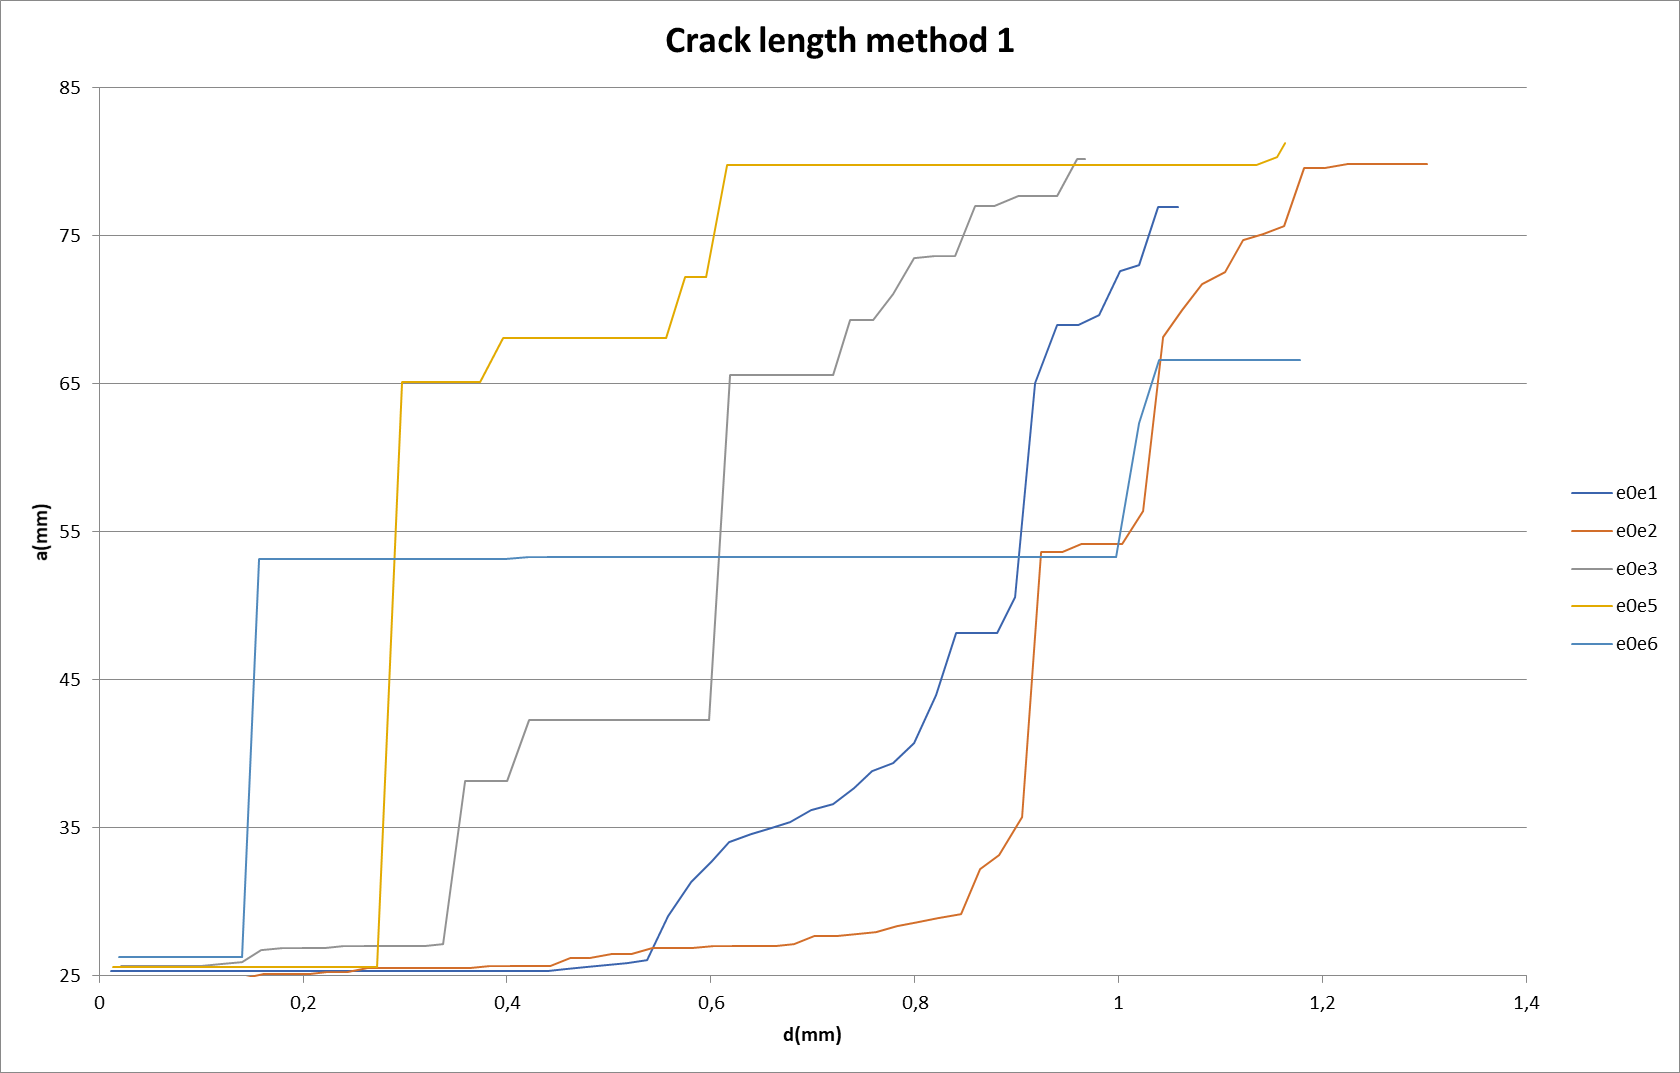
\includegraphics[width=16cm]{crack_method1}
	\caption{Crack length evolution depending on alpha}
	\label{fig:crack_method1}
\end{figure}

\begin{figure}[htp]
	\centering
	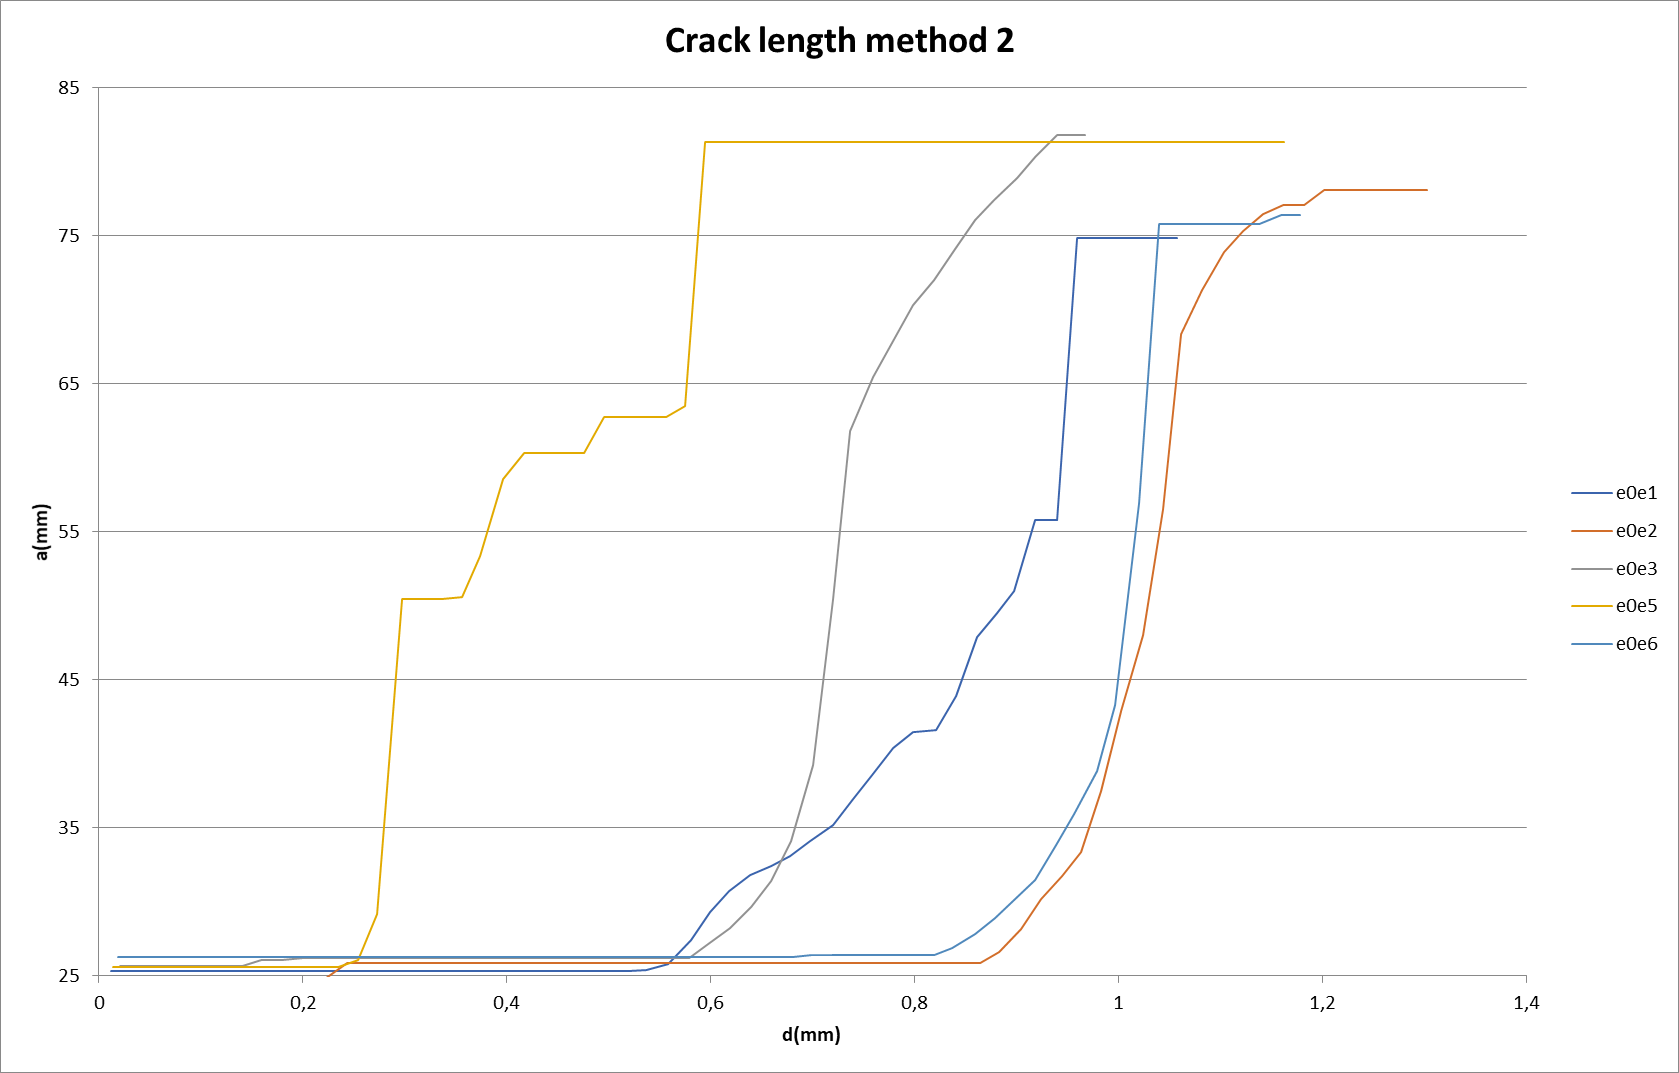
\includegraphics[width=16cm]{crack_method2}
	\caption{Crack length evolution depending on alpha}
	\label{fig:crack_method2}
\end{figure}

\section{Critical energy restitution rate}

Various methods can be used to calculate the energy restitution rate. The general formula is explained in \ref{eq:eq125}. However, it is possible to calculate complacency in different ways. One possibility, used by \cite{Odounga2018phd} and \cite{MoutouPitti2008}, is to calculate the $\Delta c$ between the starting point and the point under consideration. A second method is to determine $C(a)=m*a(t)^3+n*a(t)^2+o*a(t)+p)$ with a(t) the length of the crack.  It is then possible to use the compliance derivate by the crack length. Both methods were tested to see which would be better and finally G is calculated with $\Delta c$. In fact, the cubic function used did not pass through all the points on the graph of C as a function of a(t) and was therefore very inaccurate. The values of G obtained with this method were of the order of $10^3 J/m2$, which is too high.
The figures below show G with the 2 methods used to calculate the crack length.

\begin{figure}[htp]
	\centering
	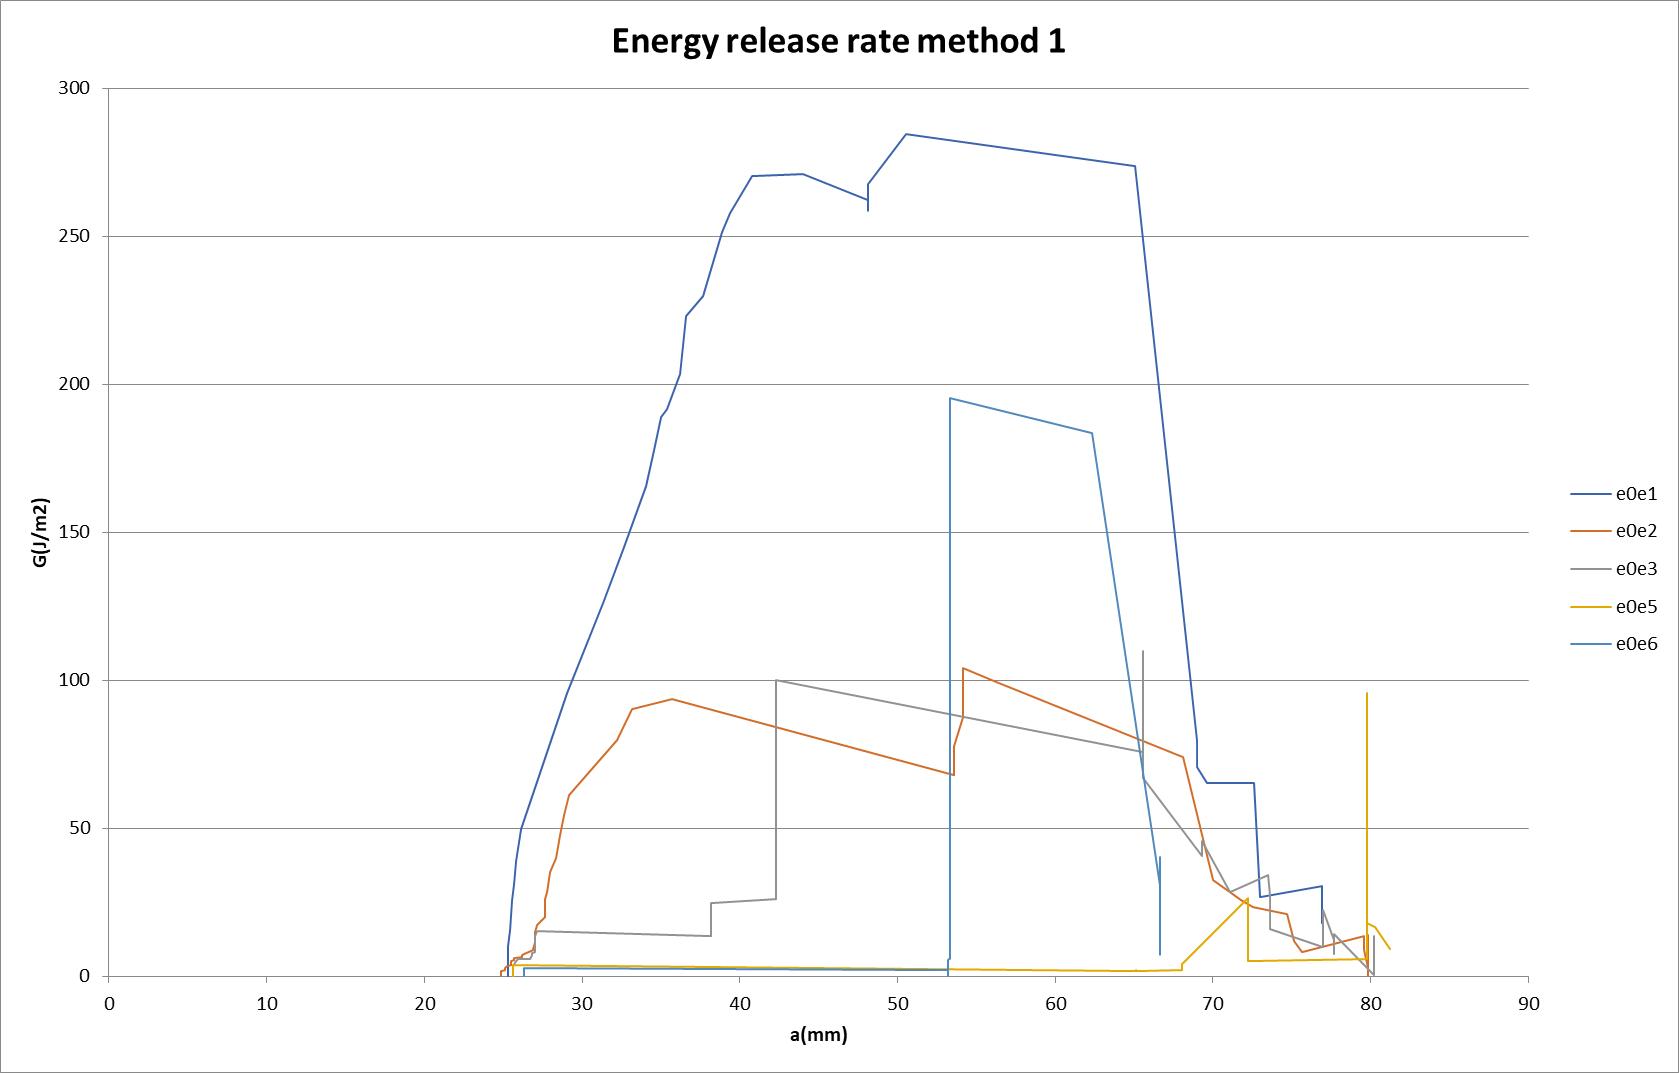
\includegraphics[width=16cm]{G_method1}
	\caption{Gmethod1}
	\label{fig:G_method1}
\end{figure}

\begin{figure}[htp]
	\centering
	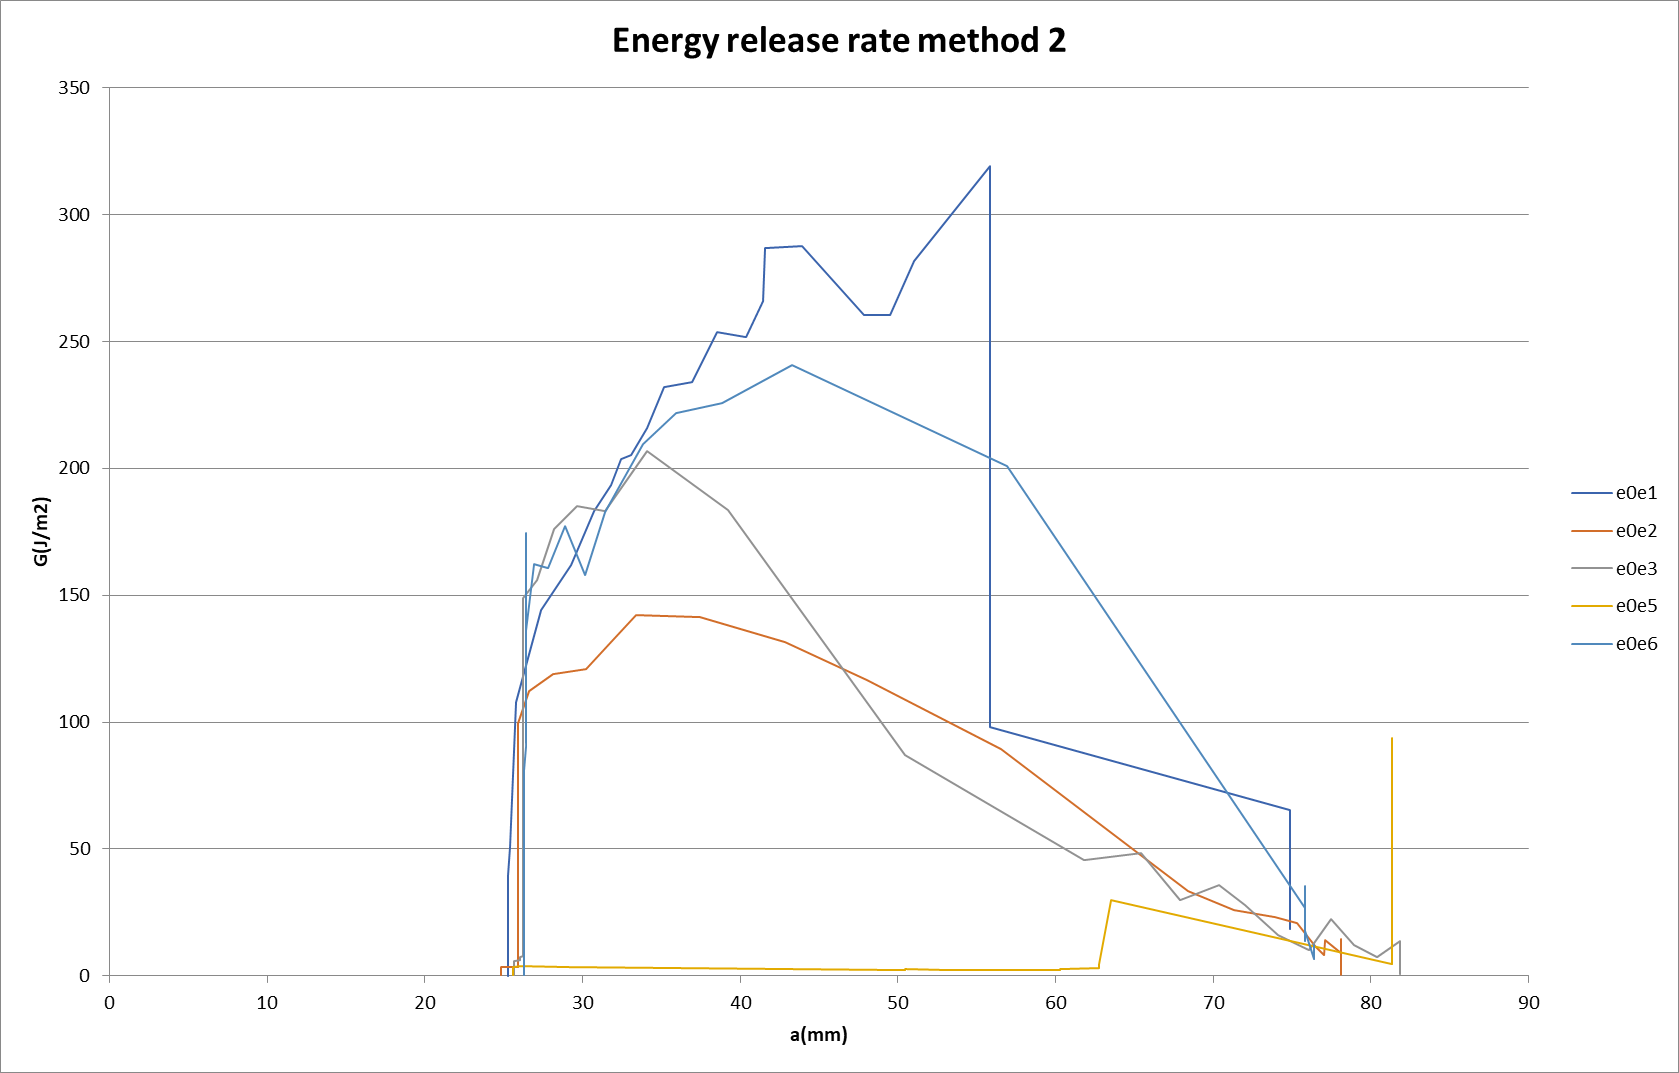
\includegraphics[width=16cm]{G_method2}
	\caption{Gmethod2}
	\label{fig:G_method2}
\end{figure}

\begin{table} \centering
	\begin{tabular}{ccccccc}
		\toprule % horizontal line at the top of the table
		&  & e0e1 & e0e2 & e0e3 & e0e5 & e0e6\\\midrule
		& Gmax method1 & 284.44 & 104.05 & 109.90 & 95.67 & 157.87 \\\midrule
		& Gmax method2 & 319.31 & 142.36 & 206.73 & 93.83 & 200.56 \\\midrule
	\end{tabular}
	\caption{Comparison of mean max G values for specimens in the literature, 2MCG: Mixed Mode Crack Growth, DCB: Double Cantilever Beam, WS: Wedge Splitting test, RL: Radial Longitudinal}
	\label{fig:fig37}
\end{table}

\section{Discussion}

Table \ref{fig:fig37} compares the different values of the maximum energy release rate obtained in this study with the literature review. These are numerous, especially in mode I. In order to provide an objective comparison, the discussion focuses on temperate species with a similar density and an initial crack oriented in the RL direction. The average maximum energy restitution rate for silver fir is shown in bold and compared to different species and different tests. There are 2MCG, DCB and wedge splitting tests.
First of all, we can see that the value of G is of the same order of magnitude as for the other species. Silver fir differs from alder by $26 \%$, Douglas fir by $34 \%$ and Padouk by $30 \%$. Moreover, in \cite{Odounga2018phd}'s work it's not uncommon to obtain values similar. In fact, his standard deviation is 2 to 3 times greater, which means that his results are more widely dispersed.
\cite{Xavieretal2014} also obtained experimental values of G=190 J/m2, which corresponds to the results obtained in this study.

\begin{table}[ht]
	\centering
	\resizebox{\textwidth}{!}{
		\begin{tabular}{cccccccc}
			\toprule % ligne horizontale en haut du tableau
			& References & Wood species & Test type & Orientation & Density & $G_{\max}(J/m^2)$ & Standard deviation \\
			\midrule
			& & \textbf{Silver fir} & \textbf{2MCG} & \textbf{RL} & \textbf{0.43} & \textbf{179} & \textbf{75} \\
			\midrule
			& \cite{Odounga2018phd} & Okoumé & 2MCG & RL & 0.39-0.5 & 317 & 160 \\
			\midrule
			& \cite{Odounga2018phd} & Iroko & 2MCG & RL & 0.56-0.7 & 323 & 200 \\
			\midrule
			& \cite{Odounga2018phd} & Padouk & 2MCG & RL & 0.7-0.88 & 255 & 200 \\
			\midrule
			& \cite{Angellier2017} & Douglas fir & DCB & RL & 0.54 & 784 &  \\
			\midrule
			& \cite{Angellier2017} & White fir & DCB & RL & 0.49 & 570 &  \\
			\midrule
			& \cite{Xavieretal2014} & Pinus Pinaster & DCB & RL & 0.543 & 270 & 64 \\
			\midrule
			& \cite{Reiterer2002} & Spruce & WS & RL & 0.479 & 337 & 47 \\
			\midrule
			& \cite{Reiterer2002} & Alder & WS & RL & 0.510 & 244 & 41 \\
			\midrule
			& \cite{Reiterer2002} & Oak & WS & RL & 0.553 & 348 & 38 \\
			\midrule
			& \cite{Reiterer2002} & Ash & WS & RL & 0.701 & 551 & 38 \\
			\bottomrule % ligne horizontale en bas du tableau
		\end{tabular}
	}
	\caption{Comparison of mean max G values for specimens in the literature, 2MCG: Mixed Mode Crack Growth, DCB: Double Cantilever Beam, WS: Wedge Splitting test, RL: Radial Longitudinal}
	\label{fig:fig37}
\end{table}

\section{Conclusion}